\subsection{\LIME metodas}\label{sec:literature:lime}

\LIME \angl{Local Interpretable Model-agnostic Explanations} -- tai lokalūs, interpretuojami \gls{ml} modelių išvesčių paaiškinimai. \gls{ml} modeliai dažnai turi būti sudėtingi (dėl to ir sunkiai, ar visiškai neinterpretuojami), nes jie aproksimuoja sudėtingus skirstinius visoje (globalioje) srityje. \LIME metodo idėja yra aproksimuoti skirstinį taip pat, kaip \gls{ml} modelis, bet žymiai mažesnėje~--~\textbf{lokalioje}~--~srityje \angl{locally faithful} aplink mus dominantį tašką (\gls{ml} modelio įvestį). Tai leidžia \LIME naudojamam aproksimacijos modeliui būti ženkliai paprastesniam, daugeliu atvejų -- tiesiniam (pvz., tiesinė regresija).
\LIME veikimo principas yra vieno pavyzdžio (įvesties $x_0$) perturbavimas taip sukuriant lokalių $x_0$ artimų įvesčių aibę $\hat{X}$. Kiekvienas $\hat{X}$ elementas pateikiamas originalaus modelio ($M$) klasifikacijai ir taip gaunama aibė $\hat{Y}$ ($\hat{X} \xrightarrow{M} \hat{Y}$). Abi aibės naudojamos surogatinio (dažniausiai tiesinio) modelio $\hat{M}$ mokymui. Tuomet \textbf{interpretuojamas paaiškinimas} yra surikiuotas pagal įtaką galutiniam $\hat{M}$ sprendimui $x_0$ komponenčių (požymių) sąrašas (pilnas arba dalinis) \cite{ribeiroWhyShouldTrust2016}.

Svarbus \LIME parametras yra branduolio plotis \angl{kernel width} \omega. \LIME mokymosi etape kiekvienai perturbuotai įvesčiai $\hat{x}_i \in \hat{X}$ priskiria svorį $a_i \propto \exp\left(-\frac{D(x_0, \hat{x}_i)}{\omega^2}\right)$. Taigi, $\omega$ turi būti parenkamas atsižvelgiant į skalę, kurioje klasifikuojami klasteriai gali būti atskiriami tiesiškai.

\LIME metodas yra paaiškinamo dirbtinio intelekto (\gls{xai}) pavyzdys. \gls{xai} gali būti naudojamas kaip \gls{ae} aptikimo strategija, jei paaiškinimai geba pastebimai atskirti \gls{ae} nuo tikrų įvesčių (pavyzdžiui, klasifikacijos paaiškinimas statistiškai reikšmingai skiriasi nuo tikrų duomenų paaiškinimų).

\subsubsection{\Glsplko{adversarial} aptikimas \gls{ids} naudojant \LIME}\label{sec:literature:defense:ids}

\glsxtrfull{ids} -- tai sistema, veikianti uždarame tinkle ir nuolat analizuojanti tinklo srautą. Vienas iš \gls{ids} įgyvendinimo būdų yra pasitelkti \gls{ml} modelius, tad šios sistemos taip pat yra pažeidžiamos \glsplkam{adversarial}. Šiame kontekste Tcydenova ir kt. pritaikė \LIME kaip \gls{ae} aptikimo strategiją. Jų siūlomas metodas \zr{fig:ids} \gls{ae} aptikimui susideda iš dviejų pagrindinių dalių \cite{tcydenovaDetectionAdversarialAttacks2021}:

\noindent
\begin{minipage}[l]{0.45\textwidth}
    \begin{enumerate}[leftmargin=*]
        \item Mokymo fazė.
        \begin{itemize}[leftmargin=*]
            \item Mokomas \gls{ml} modelis tinklo srauto klasifikavimui.
            \item Kiekvienam nekenkėjiškų mokymo duomenų pavyzdžiui pritaikomas \LIME metodas -- gaunama paaiškinimų aibė $E$, kur kiekvienas elementas yra $n$-matis vektorius, turintis $n$ svarbiausių \textbf{interpretuojamų paaiškinimų}.
            \item $E$ laikoma normalių požymių aibe.
        \end{itemize}
        \item Aptikimo fazė.
        \begin{itemize}[leftmargin=*]
            \item Išmokytas \gls{ml} modelis klasifikuoja tinklo srautą.
            \item Jei \gls{ml} modelis nustato, jog įvestis yra kenksminga -- ji tokia ir laikoma.
            \item Jei \gls{ml} modelis nustato, jog įvestis nėra kenksminga -- taikomas \LIME metodas ir gaunamas klasifikavimo paaiškinimas.
            \item Jei klasifikavimo paaiškinime figūruoja bent vienas požymis, nepriklausantis $E$ aibei -- laikoma, jog įvestis yra kenksminga.
            \item Jei visi klasifikavimo paaiškinime figūruojantys požymiai priklauso aibei $E$ -- laikoma, jog įvestis nekenksminga.
        \end{itemize}
    \end{enumerate}
\end{minipage}
\hspace{0.02\textwidth}
\begin{minipage}{0.58\textwidth}
        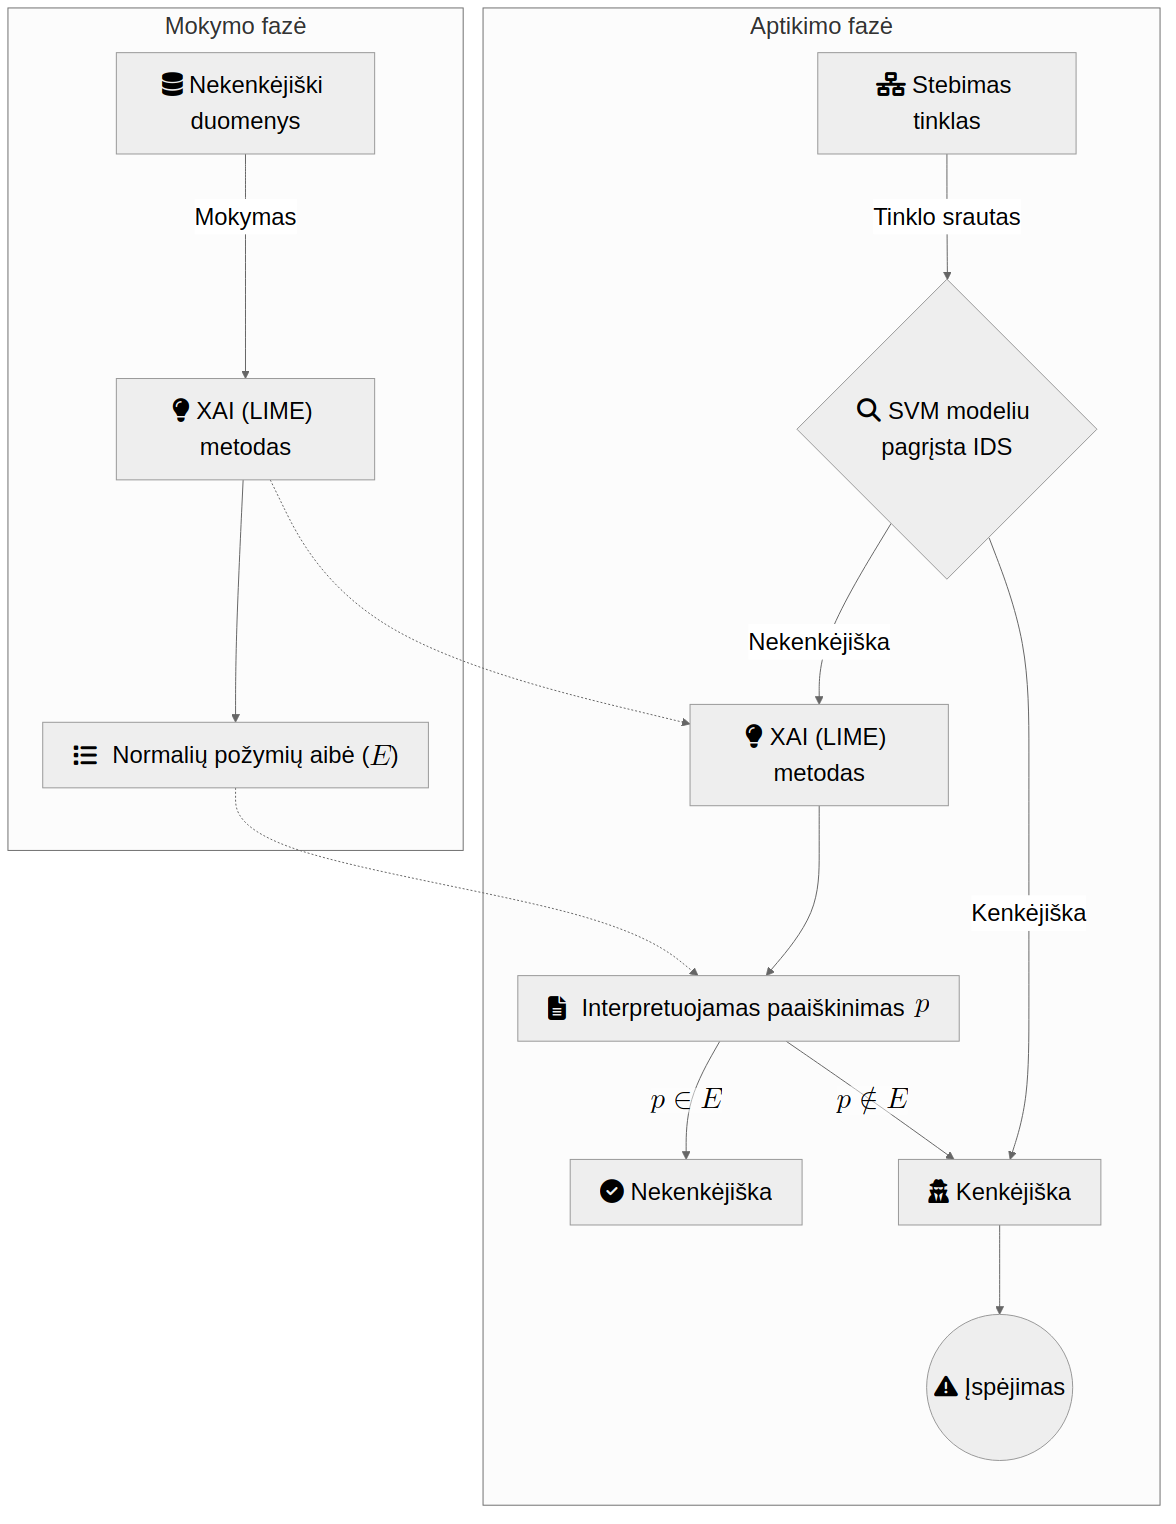
\includegraphics[width=\textwidth]{images/ids.png}
        \captionof{figure}{\LIME pritaikymas \gls{ae} aptikimui \gls{ids} (adaptuota iš \cite{tcydenovaDetectionAdversarialAttacks2021})}
        \label{fig:ids}
\end{minipage}

\break

\LIME metodo taikymas \glsplko{adversarial} aptikimui yra artimas \textbf{perkeliamumo blokavimo} \skyrius{sec:literature:defense:blocking} strategijai, tačiau šiuo atveju \LIME veikia kaip atskiras nuo pagrindinio klasifikatoriaus komponentas, tad pagrindinis \gls{ml} modelis lieka pažeidžiamas \glsplkam{adversarial}.